\documentclass[12pt,letterpaper, onecolumn]{exam}
\usepackage{amsmath}
\usepackage{amssymb}
\usepackage{nicefrac}
\usepackage{graphicx}
\usepackage{tocbasic}
\usepackage{hyperref}

\usepackage{xcolor}
\hypersetup{
	colorlinks=true,
	linkcolor=blue,
	filecolor=magenta,      
	urlcolor=cyan,
}

\usepackage[lmargin=71pt, tmargin=1.2in]{geometry}  %For centering solution box
\lhead{AP Calculus AB -- APC 4.1 -- 4.2 Assignment\\}
\rhead{Brayden Price\\}
% \chead{\hline} % Un-comment to draw line below header
\thispagestyle{empty}   %For removing header/footer from page 1
\newcommand\at[2]{\left.#1\right|_{#2}}


\DeclareNewTOC[%
type=exercise,%
types=exercises,%
name=Exercise,%
listname={List of Questions},%
tocentrystyle=tocline,%
tocentryindent=0pt,%
tocentrydynnumwidth,%
tocentrypagenumberformat=\entryprefix{page~},%
tocentrypagenumberbox=\mbox
]{exr}
\newcommand*\entryprefix[2]{#1#2}

\qformat{%
	\textbf{Question~\thequestion}%
	\addxcontentsline{exr}{exercise}{Question~\thequestion}%
	\hfill\thepoints%
}

\begin{document}

\begingroup  
    \centering
    \LARGE AP Calculus AB\\
    \LARGE AP Classroom: 4.1 -- 4.2\\[0.5em]
    \large \today\\[0.5em]
    \large Brayden Price \\
    All final solutions are \boxed{boxed} \\
\endgroup
\rule{\textwidth}{0.4pt}

\listofexercises
\clearpage

\printanswers
\renewcommand{\solutiontitle}{\noindent\textbf{Solution:}\enspace}   %Replace "Ans:" with starting keyword in solution box

\begin{questions}

%Q1
\question $$ g(x)= \begin{cases}3-x & \text { for } x<3 \\ 4 x-12 & \text { for } x \geq 3\end{cases} $$
%BEGIN_FOLD
	If $g$ is the function defined above, then $g^{\prime}(3)$ is
	\begin{parts}
		\part $-1$
		\part $0$
		\part $4$
		\part nonexistent
	\end{parts}

    \begin{solution}
          For a function to be differentiable at a point, the function must be continuous at that point.
	Check continuity of $g(x)$ at $x=3$:
	\begin{align*}
		\lim_{x\to3^-} g(x)  & = 3-3              & = 0 \\ % Left Limit 
		\lim_{x\to3^+} g(x)  & = 4(3)-12          & = 0 \\ % Right Limit
		\lim_{x\to3} g(x)    &                    & = 0  \\ % Two-sided Limit
		g(3)                 & = 4(3)-12          & = 0 \\  % Real Function
		\therefore g \text{ is continuous at } x=3
	\end{align*}
	However, the function's derivative must \emph{also} be continuous.
	Find $g^\prime(x)$:
	
	$$ g^\prime(x) =
	\begin{cases}
	-1 & \text{ for } x < 3 \\
	 4 & \text{ for } x \geq 3
	\end{cases}	
	$$
	Check continuity of $g^\prime(x)$ at $x=3$:
	\begin{align*}
		\lim_{x\to3^-} g^\prime(x)  &=  -1 \\ % Left Limit 
		\lim_{x\to3^+} g^\prime(x) &= 4 \\ % Right Limit
		\lim_{x\to3} g^\prime(x)      & \text{ does not exist.} \\ % Two-sided Limit
		\therefore g^\prime \text{ is not continuous at } x=3 \\
		\boxed{\therefore g^\prime \text{ is not differentiable at } x=3}
	\end{align*}

    \end{solution}
    
%END_FOLD

\pagebreak

%Q2
\question 
%BEGIN_FOLD
    If $ f(x) = 
\begin{cases}
	\ln x 		& \text{ for } 	    0 < x \leq 2 \\ 
	x^2 \ln 2 	& \text { for } 	2 < x \leq 4
\end{cases}
$ then $ \lim\limits_{x\to2} f(x) $ is


    \begin{parts}
	\part	$ \ln 2 $
	\part	$ \ln 8 $
	\part	$ \ln 16 $
	\part	$ 4 $
	\part nonexistent
    \end{parts}
    
    \begin{solution}
	
            \begin{align*}
		x^2 \ln 2		 &= \ln ( 2 ^  {(x ^ 2)} ) \\
		\lim_{x\to2^-} f(x)  &=  \ln 2 \\ % Left Limit 
		\lim_{x\to2^+} f(x) &= \ln (2^{(2^2)}) = \ln (2^4) = \ln 16 \\ % Right Limit
		\lim_{x\to2^+} f(x) & \neq \lim_{x\to2^-} f(x) \\ % Two-sided Limit
					 & \therefore \boxed{\lim_{x\to2} f(x) \text{ does not exist.}}
	\end{align*}
    \end{solution}
 
%END_FOLD   

\pagebreak

%Q3
\question $\frac{d}{dx} ( \tan^{-1} x + 2 \sqrt{x} ) = $	

%BEGIN_FOLD
 	\begin{parts}
		\part $ -\frac{1}{\sin ^2 x}+\frac{1}{\sqrt{x}}        $ \\
		\part $ \frac{1}{\sqrt{1-x^2}}-4 \sqrt[3]{x}           $ \\
		\part $ \frac{1}{\sqrt{1-x^2}}+\frac{1}{\sqrt{x}}   $ \\
		\part $ \frac{1}{1+x^2}-4 \sqrt[3]{x} 		       $ \\
		\part $ \frac{1}{1+x^2}+\frac{1}{\sqrt{x}}	       $
	\end{parts}

    \begin{solution}
          \begin{gather*}
		\frac{d}{dx} \left( \tan^{-1} x + 2 \sqrt{x} \right)  = \\ 
		\frac{d}{dx} \left( \tan^{-1} x \right) + \frac{d}{dx} \left( 2 \sqrt{x} \right) = \\
		\frac{\frac{d}{dx}(x)}{1+x^2} + 2 \frac{d}{dx} \left( x^{\nicefrac{1}{2}} \right) = \\
		\frac{1}{1+x^2} + 2 \left(\nicefrac{1}{2}\left(x^{\nicefrac{-1}{2}}\right)\right) = \\
		\boxed{\frac{1}{1+x^2} + \frac{1}{\sqrt{x}}}
	\end{gather*}
    \end{solution}
    
%END_FOLD

\pagebreak

%Q4
\question Let $f$ and $g$ be differentiable functions such that $f^\prime(0)=3$ and $g^\prime (0) = 7$. If $h(x)=3f(x)-2g(x)-5\cos x -3$, what is the value of $h^\prime(0)$?

%BEGIN_FOLD
    \begin{parts}
	\part	$ -8 $
	\part	$ -5 $
	\part	$ 1 $
	\part	$ 28 $
    \end{parts}
	
    \begin{solution}
	Lets start by finding $h^\prime(x)$:
	\begin{align*}
		h^\prime(x) &= 3 \frac{d}{dx} f(x) - 2 \frac{d}{dx} g(x) - 5 \frac {d}{dx} (\cos x) - \frac {d}{dx} 3 \\
		h^\prime(x) &= 3f^\prime(x) - 2g^\prime(x) + 5\sin (x) - 0
	\end{align*}
	Now we can just plug in $x$ as $0$:
	\begin{align*}
		h^\prime(0) &= 3f^\prime(0) - 2g^\prime(0) + 5\sin (0) \\
		h^\prime(0) &= 3(3) - 2(7) + 5(0) \\
		h^\prime(0) &= \boxed{-5}
	\end{align*}
    \end{solution}
%END_FOLD

\pagebreak

%Q5
\question Let $f$ be the function defined by $f(x) = e^{x} \cos x$. \\ Find the average rate of change of $f$ on the interval $ 0 \leq x \leq \pi $.

%BEGIN_FOLD
	\begin{solution}
		$$\text{AROC} = \frac{e^{\pi} \cos(\pi) - e^{0} \cos(0)}{\pi - 0} = \boxed{\frac{-e^{\pi}-1}{\pi}}$$
	\end{solution}
%END_FOLD

\pagebreak

%Q6
\question The velocity $v$, in meters per second, of a certain type of wave is given by $v(h) = 3\sqrt{h}$, where $h$ is the depth, in meters, of the water through which the wave moves. What is the rate of change, in meters per second per meter, of the velocity of the wave with respect to the depth of the water, when the depth is $2$ meters?

%BEGIN_FOLD	
	\begin{parts}
		\part $-\frac{3}{4\sqrt{2}}$
		\part $-\frac{3}{8\sqrt{2}}$
		\part $\frac{3}{2\sqrt{2}}$
		\part $\frac{3}{\sqrt{2}}$
		\part $4\sqrt{2}$
	\end{parts}

	\begin{solution}
		The  question asks us to find the rate of change of the velocity of the wave $v$ with respect to the depth of the water $h$, which is, in derivative terms, $\frac{dv}{dh}$. \\
		Find $\frac{dv}{dh}$:
		\begin{align*}
			\frac{dv}{dh} 3\sqrt{h} & = 3 \frac{dv}{dh} h^{\nicefrac{1}{2}} \\
			3 \frac{dv}{dh} h^{\nicefrac{1}{2}} & = 3 \left(\frac{1}{2}\right) h^{\nicefrac{-1}{2}} \\
			3 (\frac{1}{2}) h^{\nicefrac{-1}{2}} & = \frac{3}{2\sqrt{h}}
		\end{align*}
		Find $\at{\frac{dv}{dh}}{h=2}$:
			$$\boxed{\frac{3}{2\sqrt{2}}}$$
	\end{solution}
%END_FOLD

\pagebreak

%Q7
\question The function $t=f(S)$ models the time, in hours, for a sample of water to evaporate as a function of the size $S$ of the sample, measured in milliliters. What are the units for $f^{\prime\prime}(S)$?
%BEGIN_FOLD
	\begin{parts}
		\part hours per milliliter
		\part milliliters per hour
		\part hours per milliliter per milliliter
		\part milliliters per hour per hour
	\end{parts}

	\begin{solution}
		The units of the first derivative $f^{\prime}(S)$ can be found by dividing the units of the output by the units of the input: 
		$$\frac{hours}{milliliter}$$
		To find the second derivative's units, we apply the same process to the first derivative:
		$$\frac{\frac{hours}{milliliter}}{milliliter}$$
		This can also be written as \boxed{\textbf{hours per milliliter per milliliter}}.
	\end{solution}
%END_FOLD

\pagebreak

%Q8
\question
%BEGIN_FOLD
	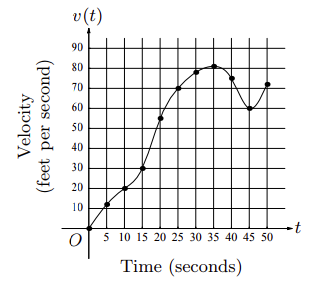
\includegraphics[width=0.5\linewidth]{Question8-001}
	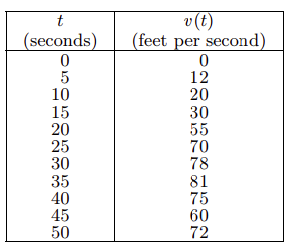
\includegraphics[width=0.5\linewidth]{Question8-002} \\
	The graph of the velocity $v(t)$, in ft/sec, of a car traveling on a straight road, for $0 \leq t \leq 50$, is shown above. A table of values for $v(t)$, at $5$ second intervals of time $t$, is shown to the right of the graph. \\
	Find one approximation for the acceleration of the car, in ft/sec\textsuperscript{2}, at $t = 40$. Show the computations you used to arrive at your answer.
	
\begin{solution}
	Acceleration at $t=40$ can be estimated using the Average Rate of Change over $35 \leq t \leq 45$:
	$$AROC=\frac{v(45)-v(35)}{45-35}=\frac{60-81 \text{ ft/sec}}{10 \text{ sec}}= \frac{-21\text{ ft/sec}}{10 \text{ sec}} = \boxed{-2.1 \text{ ft/sec\textsuperscript{2}}}$$
\end{solution}
%END_FOLD

\pagebreak

%Q9
\question
%BEGIN_FOLD
The position of a particle moving along a straight line at any time t is given by $s(t)=t^2+4t+4$. What is the acceleration of the particle when $t=4$?

\begin{solution}
	For any position function $s(t)$, $\frac{d}{dt} s(t) = v(t)$ where $g(t)$ is the corresponding velocity equation. For any velocity equation $v(t)$, $\frac{d}{dt} v(t) = a(t)$, where $a(t)$ is the corresponding acceleration equation. \\
	Find $v(t)$:
	$$v(t)=\frac{d}{dt} s(t) =\frac{d}{dt} (t^2+4t+4) = 2t+4 $$
	Find $a(t)$:
	$$a(t)=\frac{d}{dt} v(t) =\frac{d}{dt} (2t+4) = 2 $$
	Find $a(4)$ (evaluate $\at{\frac{d^{2}}{dt^{2}}s(t)}{t=4}$):
	$$\boxed{a(4)=2}$$
\end{solution}

%END_FOLD

\pagebreak

%Q10
\question
%BEGIN_FOLD
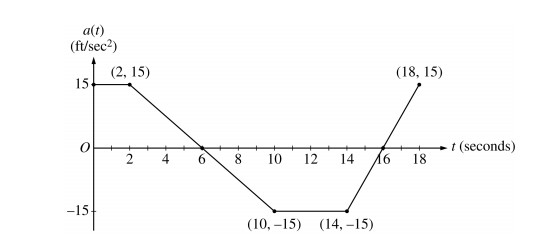
\includegraphics[width=0.7\linewidth]{Question10-001} \\
A car is traveling on a straight road with velocity $55$ ft/sec at time t = 0. For $0 \leq t \leq 18$ seconds, the car's acceleration $a(t)$, in ft/sec\textsuperscript{2}, is the piecewise linear function defined by the graph above. \\
Is the velocity of the car increasing at t = 2 seconds? Why or why not?
\begin{solution}
	When $t=2$, $a(t) > 0$, indicating that the derivative $\frac{dv}{dt}$ of velocity with respect to time is positive. When a derivative is positive at a point, this indicates that the original function must be increasing at this point. \\ \boxed{\text{Therefore, the velocity at this time $t=2$ seconds must be increasing.}} 
\end{solution}
%END_FOLD

\pagebreak

%Q11
\question
%BEGIN_FOLD
The penguin population on an island is modeled by a differentiable function $P$ of time $t$, where $P(t)$ is the number of penguins and $t$ is measured in years for $0 \leq t \leq 40$. There are $100,000$ penguins on the island at time $t = 0$. The birth rate for the penguins on the island is modeled by:
$$B(t) = 1000e^{0.06t} \text{ penguins per year}$$ 
and the death rate for the penguins on the island is modeled by:
$$D(t)=250e^{0.1t} \text{ penguins per year.}$$
What is the rate of change for the penguin population on the island at time $t = 0$?
\begin{solution}
	The rate of change of the penguin population at a particular time $t$ can be modeled by the derivative of the penguin population function $P(t)$. \\
	We can create $P^\prime(t)$ by subtracting the death rate function $D(t)$ from the birth rate function $B(t)$:
	$$P^\prime(t)=B(t)-D(t)$$
	$$P^\prime(0)=B(0)-D(0) = 1000-250 = \boxed{750 \text{ penguins per year}}$$
\end{solution}

%END_FOLD

\pagebreak

%Q12
\question
%BEGIN_FOLD
The tide removes sand from Sandy Point Beach at a rate modeled by the function $R$, given by $R(t)=2+5\sin(\frac{4\pi t}{25})$. \\
A pumping station adds sand to the beach at a rate modeled by the function $S$, given by $S(t)=\frac{15t}{1+3t}$. \\
Both $R(t)$ and $S(t)$ have units of cubic yards per hour and $t$ is measured in hours for $0 \leq t \leq 6$. At time $t = 0$, the beach contains $2500$ cubic yards of sand. \\
Find the rate at which the total amount of sand on the beach is changing at time $t = 4$.

\begin{solution}
	The net rate at which sand is changing at a time $t$ can be given by the following function $N(t)$:
	$$N(t)=S(t)-R(t)$$
	\emph{(assuming that sand is only being added by the pumping station at a rate modeled by $S(t)$ and removed by the tide at a rate modeled by $R(t)$.)} \\
	Evaluate $N(4)$:
	$$N(4)=S(4)-R(4)=4.6153-2.1754=\boxed{2.4399 \text{ cubic yards per hour}}$$
	{\textbf{\color{red} {\large \underline{NOTE}}: This does not match the numerical solution given on AP Classroom, and I don't know why. Will be asking Mr. Reid about it tomorrow. (The process does match the one on AP Classroom.)}}
\end{solution}
%END_FOLD

\pagebreak

%Q13
\question
%BEGIN_FOLD
A differentiable function $f$ has the property that $f(5)=3$ and $f^\prime(5)=4$. What is the estimate for 
using the local linear approximation for $f$ at $x = 5$?

\begin{solution}
	Write tangent line at $x=5$: \\
	Point is $(5,3)$ \\
	Slope $m=4$ \\
	\begin{align}
		y-y_{1} &= m(x-x_1) \\
		y-3 &= 4(x-5) \\
		y &= 4(x-5) + 3
	\end{align}
	Plug in $x=4.8$:
	\begin{align}
		y &= 4(4.8-5) + 3 \\
		y &= \boxed{2.2}
	\end{align}
\end{solution}
%END_FOLD

\end{questions}
\end{document}